\documentclass[11pt]{article}
\usepackage[margin=0.78in]{geometry}
\usepackage[T1]{fontenc}
\usepackage[utf8]{inputenc}
\usepackage{lmodern}
\usepackage{microtype}
\usepackage{amsmath,amssymb,mathtools}
\usepackage{booktabs,longtable,tabularx,array}
\usepackage{graphicx}
\usepackage{enumitem}
\usepackage{xcolor}
\usepackage[colorinlistoftodos,textsize=small]{todonotes}
\usepackage{xurl}
\usepackage{hyperref}

\hypersetup{colorlinks=true,linkcolor=black,citecolor=blue!55!black,urlcolor=blue!65!black}
\setlength{\parindent}{0pt}
\setlength{\parskip}{4.5pt}
\renewcommand{\arraystretch}{1.10}
\setlist[itemize]{leftmargin=1.35em,itemsep=1.5pt,topsep=2pt}
\setlist[enumerate]{leftmargin=1.55em,itemsep=1.5pt,topsep=2pt}
\newcolumntype{Y}{>{\raggedright\arraybackslash}X}

\newcommand{\Reported}{\textsc{reported}}
\newcommand{\Measured}{\textsc{measured}}
\newcommand{\Derived}{\textsc{derived}}
\newcommand{\Fitted}{\textsc{fitted}}
\newcommand{\Proxy}{\textsc{proxy}}
\newcommand{\Scenario}{\textsc{scenario}}
\newcommand{\Benchmark}{\textsc{external benchmark}}
\newcommand{\NotIdentified}{\textsc{not identified}}
\newcommand{\Strong}{\textsc{strong support}}
\newcommand{\Partial}{\textsc{partial}}
\newcommand{\Pending}{\textsc{pending}}

\title{\textbf{Network-Based Planning for Data Centers}\\
\large Canonical Scientific Model, Evidence, Validation Status, and Research Path}
\author{Internal living scientific document}
\date{Status snapshot: August 27, 2026}

\begin{document}
\maketitle
\vspace{-0.8em}

\begin{center}
\small
\textit{Purpose.} This is the single living scientific source of truth for the project. It records the current research objective, mathematical model, evidence supporting each link, validation status, what remains unidentified, and the next scientific gates. Accepted conclusions are written as normal text; unresolved items are marked only by short TODOs. Historical wording belongs in git history and archived drafts, not in this document.
\end{center}

% ================================================================
\section{North star: the scientific question}
% ================================================================

The project is a \textbf{coupled infrastructure--natural-resource planning problem}. The goal is not merely to estimate a data center's PUE, WUE, or annual footprint. The goal is to determine how data-center demand, technology, siting, and source choices interact with electricity systems and shared water resources, and whether accounting for those interactions changes optimal planning and policy.

The canonical causal chain is
\[
\boxed{\begin{gathered}
\text{workload / compute demand}
\rightarrow P^{IT}
\rightarrow \{P^{fac},\,W^{cond}\}\\
\rightarrow \{\text{grid},\,W^{with}\text{ by source}\}
\rightarrow \{\mathrm{CO_2},\,\text{generator water},\,q^{gw}\}\\
\rightarrow \text{groundwater state and competing-sector impacts}
\rightarrow \text{operations, siting, and policy}.
\end{gathered}}
\]

The J-WAFS project provides the north-star structure: a reduced groundwater-network model (Thrust A), infrastructure planning coupled to groundwater and competing agricultural/municipal demands (Thrust B), and policy/decentralization mechanisms (Thrust C) \cite{jwa}. The PSCC model is the natural static planning baseline: it already trades off cost, carbon, water-scarcity footprint, renewables, and spatial equity, but its water representation is static rather than a dynamic physical resource \cite{pscc}.

The strongest prospective research result is therefore not ``a more detailed data-center simulator.'' It is:
\[
\boxed{\parbox{0.88\linewidth}{\centering
Static water-scarcity rankings and dynamic groundwater-network impacts can disagree, and this disagreement can change optimal data-center siting, cooling/source choices, multi-sector burdens, or policy conclusions.}}
\]

\textbf{Role of current empirical work.} Prineville is a site-specific public-data test bed for electricity, water, grid, permitting, pumping, and groundwater layers. M100, Lei--Masanet, Frontier, and the modern IT-power datasets are external validation sources used to identify defensible generic model structure. Prineville is not the ``generic data center,'' and external benchmark coefficients are not transferred to it without a justified bridge.


% ----------------------------------------------------------------
% Living Figure 1: canonical project architecture.
% If the named PDF exists, it is used automatically; otherwise the
% self-documenting placeholder below keeps this file fully compilable.
% ----------------------------------------------------------------
\begin{figure}[!htbp]
\centering
\IfFileExists{img/fig_canonical_project_architecture.pdf}{%
  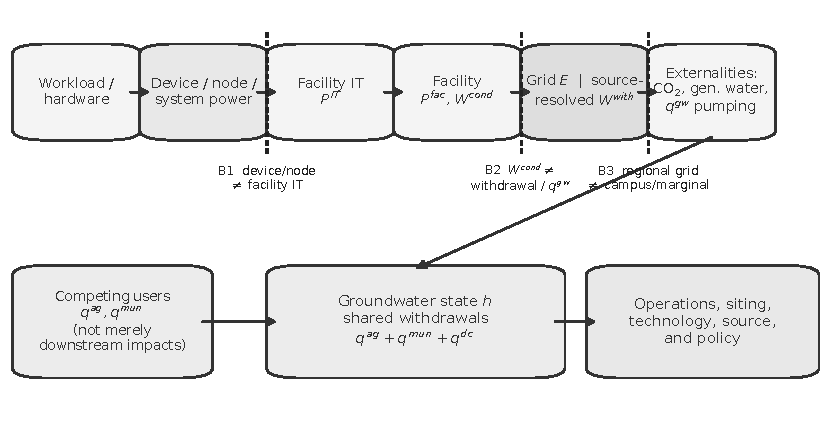
\includegraphics[width=0.96\linewidth]{img/fig_canonical_project_architecture.pdf}%
}{%
  \fbox{\begin{minipage}[c][2.35in][c]{0.90\linewidth}
  \centering
  \textbf{PLACEHOLDER --- Canonical coupled-system architecture}\\[0.7em]
  Workload / hardware $\rightarrow$ facility IT power
  $\rightarrow$ facility electricity + conditioning water
  $\rightarrow$ grid + source-resolved withdrawal
  $\rightarrow$ emissions + generator water + groundwater pumping
  $\rightarrow$ dynamic groundwater state + competing users
  $\rightarrow$ siting / technology / source / policy decisions.\\[0.7em]
  Show explicit boundary breaks at device/node $\rightarrow$ facility IT,
  conditioning water $\rightarrow$ withdrawal/source, and regional grid
  $\rightarrow$ campus or marginal attribution.
  \end{minipage}}%
}
\caption{\textbf{Canonical coupled-system architecture.}
The project links compute demand to facility energy and water requirements,
source-resolved infrastructure demands, dynamic groundwater consequences,
and ultimately planning and policy decisions. Boundary markers identify
mappings that must be estimated or externally identified rather than assumed.}
\label{fig:canonical_architecture}
\end{figure}

% ================================================================
\section{Canonical model hierarchy}
% ================================================================

\subsection{Indices, scales, and boundaries}

Let $\ell\in\mathcal L$ denote candidate data-center locations, $k\in\mathcal K$ facility/cooling archetypes, $t$ an operational interval (typically hourly for planning), $m$ a groundwater management period (typically monthly/seasonal), and $i\in\mathcal N$ groundwater nodes or response units.

The project keeps power and energy distinct:
\[
E_t=P_t\Delta t.
\]
Operational/facility quantities may be hourly, while groundwater states should initially be monthly or seasonal. Annual operator disclosures do not identify hourly internal states.

\subsection{Workload / hardware $\rightarrow$ facility IT power}

A general compute-side model is
\[
P^{IT,node}_{jt}
=\mathcal P_h(x_{jt},u_{jt},\text{hardware}_h,\text{workload}_{jt}),
\]
followed by an explicit boundary map
\[
P^{IT,fac}_{\ell t}
=\mathcal A_h\!\left(\{P^{IT,node}_{jt}\}_{j\in\ell};\theta_h^{IT}\right).
\]

This separation is mandatory. M100 shows that summed qualified node power tracks the canonical facility IT meter but covers only roughly $74.5$--$80.9\%$ of that boundary; the residual is a meter/boundary gap, not a transferable ``PSU efficiency.'' The modern AI IT-power experiment therefore keeps device, node/system, and facility-IT boundaries separate.

\textbf{Current status:} no generic modern-AI workload $\rightarrow P^{IT,fac}$ map is yet validated. NLR, the 2026 H100/B200 dataset, MLPerf Power, and the frozen M100 boundary result form the predeclared validation stack.

\subsection{Facility IT $\rightarrow$ facility electricity}

The canonical accounting identity is
\[
\boxed{P^{fac}_{\ell t}=P^{IT}_{\ell t}+P^{cool}_{\ell t}+P^{aux}_{\ell t}.}
\]
PUE is a derived KPI,
\[
PUE_{\ell t}=\frac{P^{fac}_{\ell t}}{P^{IT}_{\ell t}},
\]
not an independently sampled primitive.

For \textbf{planning}, the current highest-confidence reduced model is an archetype intensity form
\[
\boxed{P^{fac}_{\ell t}
=P^{IT}_{\ell t}\,PUE_k(\mathbf w_{\ell t},\theta_k),}
\]
where $\mathbf w$ is a physically relevant weather vector and $\theta_k$ contains archetype-specific facility parameters. Equivalently,
\[
P^{nonIT}_{\ell t}=P^{IT}_{\ell t}\bigl[PUE_k(\mathbf w_{\ell t},\theta_k)-1\bigr].
\]

This form is motivated jointly by measured M100 evidence (weather matters), Frontier evidence (IT load matters for accessory/cooling power), and the Lei--Masanet climate/technology intensity model. It does \emph{not} assert universal coefficients or universal weather variables.

With variable IT load, annual PUE must be energy-weighted:
\[
\boxed{PUE_y=\frac{\sum_{t\in y}P^{fac}_t\Delta t}{\sum_{t\in y}P^{IT}_t\Delta t}.}
\]

A more detailed operational model may introduce a latent state
\[
s_{t+1}=g_k(s_t,P^{IT}_t,\mathbf w_t),\qquad
P^{cool}_t=f_k(P^{IT}_t,\mathbf w_t,s_t),
\]
but M100 does not identify a generic state equation, and its tested simple recursive dynamic model was not successful. Dynamics should be added only when independent evidence and decision relevance justify them.

\subsection{Facility operation $\rightarrow$ conditioning water $\rightarrow$ source water}

Lei--Masanet currently provides the cleanest generic facility-side water quantity:
\[
\boxed{W^{cond}_{\ell t}
=E^{IT}_{\ell t}\,WUE_k(\mathbf w_{\ell t},\theta_k).}
\]
Here $W^{cond}$ is modeled onsite conditioning-water use. The upstream total includes tower evaporation, drift/windage, draw-off/blowdown, adiabatic/direct evaporative cooling, and humidification.\par
It is \textbf{not automatically source withdrawal, total consumption, return flow, or groundwater pumping}.

The source-accounting bridge therefore remains explicit:
\[
\boxed{
W^{cond}_{\ell t}+W^{other}_{\ell t}
\xrightarrow{\ \Psi_k\ }
\{W^{with}_{\ell t},W^{cons}_{\ell t},W^{return}_{\ell t}\}
\rightarrow \{W^{municipal},W^{direct\,gw},W^{reuse},\ldots\}.
}
\]
The exact map $\Psi_k$ depends on technology, reuse/reclaimed supply, blowdown destination, non-cooling uses, and storage. This bridge is not yet identified generically.

For variable IT load,
\[
\boxed{WUE_y=\frac{\sum_{t\in y}W^{cond}_t}{\sum_{t\in y}E^{IT}_t}.}
\]
PUE and WUE should be generated from the \emph{same} archetype, weather, and facility-parameter draw so that energy--water tradeoffs remain physically coherent.

\subsection{Source-resolved withdrawal $\rightarrow$ groundwater forcing}

Let $\theta^{gw}_{\ell k t}$ denote the identified fraction of site withdrawal supplied by groundwater. Then
\[
W^{gw}_{\ell k t}=\theta^{gw}_{\ell k t}W^{with}_{\ell k t}.
\]
A spatial crosswalk $M_{i\ell}$ maps site/source withdrawals to groundwater response units. Aggregated to groundwater period $m$,
\[
\boxed{q^{dc}_{im}
=\sum_{\ell,k}M_{i\ell}\sum_{t\in m}W^{gw}_{\ell k t}.}
\]
This is the correct bridge for groundwater modeling. Neither ISO WUE nor Lei--Masanet $W^{cond}$ should be inserted directly as $q^{dc}$.

\subsection{Groundwater dynamics}

The target reduced-order state model is
\[
\boxed{h_{m+1}
=A h_m+B_RR_m-B_Q\bigl(q^{ag}_m+q^{mun}_m+q^{dc}_m\bigr)+\varepsilon_m,}
\]
where $h_m$ is a groundwater state/head vector, $R_m$ recharge/background forcing, and $q^{ag},q^{mun},q^{dc}$ sectoral withdrawals. A full MODFLOW-style model is a calibration/validation benchmark when data permit; the planning model should remain reduced-order and interpretable \cite{modflow,harou}.

\textbf{Current Prineville status:} a common-datum spatial/network state is not identified. The immediate empirical target is a within-well physically signed anomaly
\[
\tilde h_{i,m}=-(BLS_{i,m}-\overline{BLS}_i),
\]
used only to test whether antecedent pumping adds chronological predictive information beyond seasonality and trend.

\subsection{Grid externalities}

Regional accounting quantities remain separate from campus and marginal-response quantities. For a regional average benchmark,
\[
\widehat{CO}_{2,t}=CI_tE^{grid}_t,\qquad
\widehat W^{ind}_t=EWIF_tE^{grid}_t.
\]
These are useful for accounting/context but do not identify the exact generators serving a campus or the marginal power-system response to the data-center load.

% ================================================================
\section{Planning model and model-fidelity ladder}
% ================================================================

The PSCC formulation is the static baseline. The project should preserve its tractable planning structure while progressively replacing static environmental coefficients with validated endogenous response layers.

A stylized decision vector may contain siting capacity $x_\ell$, archetype choice $z_{\ell k}$, IT service $a_{\ell kt}$, grid energy, renewables, and eventually source-water choices. The first dynamic-groundwater prototype should stay deterministic and linear/convex where possible, with agriculture and municipalities treated as explicit competing withdrawals.

The recommended fidelity ladder is:

\begin{center}
\small
\begin{tabularx}{0.96\linewidth}{@{}p{0.14\linewidth}p{0.31\linewidth}Y@{}}
\toprule
\textbf{Level} & \textbf{Facility/water representation} & \textbf{Purpose} \\
\midrule
$M_0$ & Fixed PUE + fixed water coefficient / scarcity factor & Reproduce the PSCC-style baseline and quantify what the richer model changes. \\
$M_1$ & Climate--technology archetype: $P^{fac}=P^{IT}PUE_k(\mathbf w)$, $W^{cond}=E^{IT}WUE_k(\mathbf w)$ + explicit source bridge & Preferred planning model if the Masanet annual/RNG gate passes. \\
$M_2$ & Higher-fidelity part-load / thermal / state dynamics & Use only for replay/validation or if it materially changes decisions/constraints. \\
\bottomrule
\end{tabularx}
\end{center}

Model complexity should be judged by \textbf{decision relevance}, not only predictive fit. If $J_{HF}$ denotes evaluation in the highest-fidelity available emulator, compare
\[
Regret(M_r)=J_{HF}(x^*_{M_r})-\min_xJ_{HF}(x),
\]
along with changed site rankings, cooling/source choices, groundwater violations, capacity violations, and equity outcomes. If $M_1$ and $M_2$ produce the same decisions with negligible regret, retain $M_1$ in optimization.

% ================================================================
\section{Evidence and validation status}
% ================================================================

The project uses a strict provenance vocabulary. \Reported{} and \Measured{} quantities are used only at their stated boundaries; \Derived{}, \Fitted{}, \Proxy{}, and \Scenario{} quantities are never presented as direct telemetry. External datasets are \Benchmark{} evidence used to test structure or archetype behavior, not to transfer site-specific coefficients.


% ----------------------------------------------------------------
% Living Figure 2: evidence-to-model validation map.
% ----------------------------------------------------------------
\begin{figure}[!htbp]
\centering
\IfFileExists{img/fig_evidence_to_model_map.pdf}{%
  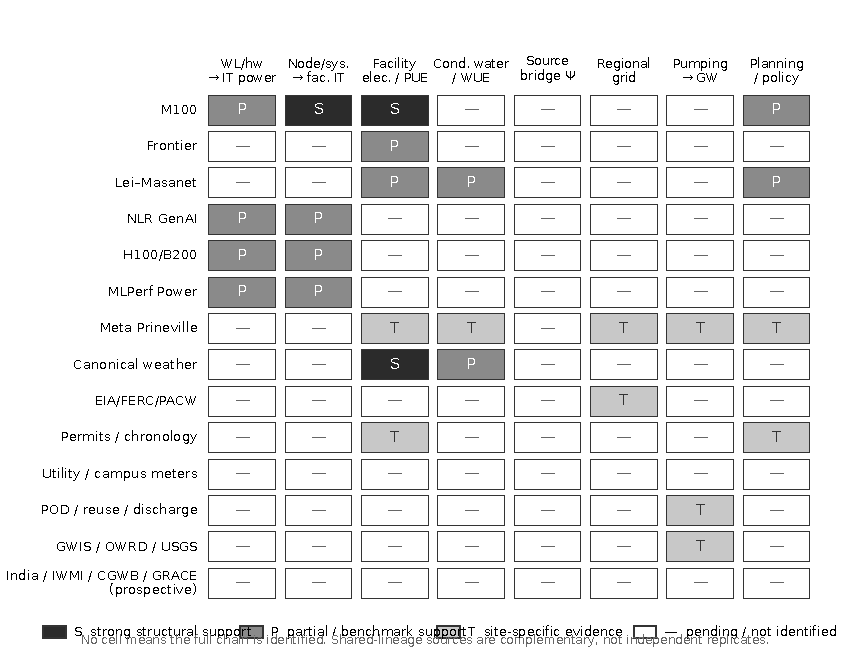
\includegraphics[width=0.98\linewidth]{img/fig_evidence_to_model_map.pdf}%
}{%
  \fbox{\begin{minipage}[c][2.45in][c]{0.92\linewidth}
  \centering
  \textbf{PLACEHOLDER --- Evidence-to-model validation map}\\[0.7em]
  Columns: workload/hardware $\rightarrow$ facility IT $\rightarrow$
  facility electricity/water $\rightarrow$ source water/grid $\rightarrow$
  groundwater state $\rightarrow$ planning/policy.\\[0.6em]
  Rows: M100; Frontier; Lei--Masanet; NLR/H100/B200/MLPerf;
  Meta Prineville; PacifiCorp/EIA/FERC; City/POD/reuse/discharge;
  GWIS/OWRD/USGS; future India/IWMI/CGWB/GRACE evidence.\\[0.6em]
  Mark cells as structural validation, partial evidence, site-specific
  calibration, external benchmark, pending, or not identified.
  \end{minipage}}%
}
\caption{\textbf{Evidence map for the coupled model.}
No single dataset identifies the complete causal chain. Independent sources
validate different model boundaries and should be combined only where their
quantities, provenance, and system definitions are compatible.}
\label{fig:evidence_map}
\end{figure}

\subsection{M100 ExaData: closed structural benchmark}

M100 is the strongest measured benchmark for the missing internal facility layer \cite{m100}. The v3 closure uses nine qualified full-facility months (Apr--Dec 2021) and eight expanding chronological folds.

\begin{center}
\scriptsize
\begin{tabularx}{\linewidth}{@{}p{0.23\linewidth}p{0.40\linewidth}Y@{}}
\toprule
\textbf{Question} & \textbf{Result} & \textbf{Canonical implication} \\
\midrule
Facility boundary & Canonical facility/IT meters are internally consistent; validated cooling components explain about $95.5$--$98.2\%$ of M100 non-IT energy. & Use $P^{fac}=P^{IT}+P^{cool}+P^{aux}$; do not transfer the M100 cooling share. \\
Weather & Adding weather to affine IT load improves held-out MAE in $8/8$ expanding folds (about $42\%$ mean improvement) and in $7/9$ fixed within-month tests. & Weather must be explicit in the planning facility model. \\
IT$\times$weather & The predeclared $P^{IT}\times T_{wb}$ interaction achieves $\ge5\%$ MAE improvement in $0/8$ folds. & Do not require this interaction in the minimum generic model. \\
Free-cooling state & Regime/state enrichment is stably useful in only $2/8$ folds and worsens most later folds. & Do not expose M100 \texttt{Free\_Cooling\_Status} as a required generic input. \\
Temporal memory & Static residuals are strongly persistent; a one-step oracle helps, but the tested recursive D1 model is worse than the static weather model in $7/8$ folds. & Temporal dependence exists, but the operational state equation is not identified. \\
Node $\rightarrow$ facility IT & Summed qualified node power tracks $Tot\_ict$ but covers only about $74.5$--$80.9\%$. & Preserve an explicit node/system $\rightarrow$ facility-IT boundary map. \\
Water & No independently verified site makeup/withdrawal/consumption meter. & M100 cannot identify WUE or groundwater pumping. \\
\bottomrule
\end{tabularx}
\end{center}

Additional QC limits remain part of the record: the processed tables support strong energy-integral/gap robustness but do not permit reconstructing the requested raw $\ge90\%$ source-sample coverage filter; October's reported-PUE channel is anomalous while canonical power meters remain usable; the 2026 M100 dynamic-model code is same-data triangulation and had a numerical reproduction discrepancy, so it is not independent confirmation.

\textbf{Status:} M100 is scientifically closed/frozen. No further M100 model search is planned.

\subsection{Lei--Masanet: facility energy--water archetype validation}

Lei--Masanet 2022 is the current archetype/intensity backbone candidate \cite{lei2022}. The first audit is complete and intentionally did not inspect the frozen Meta 2023--2024 water holdout.

High-confidence findings from the first run are:
\begin{itemize}
\item The upstream implementation is fundamentally \textbf{IT-normalized}: $P^{IT}=1$ internally. Instrumented relative-load tests at $0.5/1/2$ leave PUE/WUE invariant while absolute components scale approximately linearly. It therefore identifies climate/technology intensities, not nonlinear IT part-load behavior.
\item The modeled water quantity is onsite conditioning-water use (tower evaporation, drift/windage, draw-off/blowdown, adiabatic cooling, humidification). Source withdrawal, separate total consumption, return/discharge, and source shares remain unidentified.
\item A controlled climate/archetype grid completed without non-finite outputs, PUE$<1$, negative physical water components, or accounting-identity failures, and shows plausible electricity--water tradeoffs.
\item Reproduction is \textbf{partial}: all COP models run in the pinned environment with a documented compatibility shim; demo WUE reproduces, but the stored demo PUE does not. The annual published envelope is therefore the correct validation target.
\end{itemize}

\textbf{Current gate (running at the verified status snapshot).} Six case$\times$climate cells were predeclared before inspecting errors and span wet/waterside, air-cooled, DX, economizer, hot/humid, and cold regimes. Each uses the paper-style $50$ LHS facility samples $\times8760$ TMY hours. Hidden upstream RNG is separately compared with facility-parameter uncertainty. Adapter tests and a Prineville-2022-weather translation are blocked unless the annual/RNG gate passes. The Meta 2023--2024 water holdout remains unread.

\todo[inline,backgroundcolor=gray!10,bordercolor=gray!50,linecolor=gray!50]{Replace this running status with the canonical FOLLOWUP\_V1\_STATUS.json / FOLLOWUP\_V1\_SUMMARY.md result when the Slurm DAG finishes. If the gate fails, retain Lei--Masanet only as qualitative archetype evidence; do not force an adapter.}

\subsection{Frontier: independent measured power/thermal evidence}

Frontier provides a different liquid-cooled facility with measured compute/accessory power and coolant variables \cite{frontier}. In nine expanding chronological folds, an affine model $P^{accessory}=a+bP^{IT}$ improves mean MAE from about $0.0601$ to $0.0476$ MW (about $21\%$) versus a constant baseline and improves in all nine folds. Adding a contemporaneous measured thermal oracle does not add stable further skill.

The first time-grid audit confused null timestamps with missing expected 10-minute intervals. Roughly $2691$ expected intervals are absent, consistent with known outages. Gap-safe time/energy QC is therefore being finalized; pointwise chronological model comparisons are expected to remain unchanged. Reconstructing $\rho c_p\dot V\Delta T$ reproduces the paper's supplied waste-heat calculation and is not independent conservation validation.

\textbf{Canonical implication:} independent measured support that IT load materially affects facility accessory/cooling power; Frontier does not identify site water withdrawal/WUE or universal coefficients.

\subsection{Modern AI workload / hardware $\rightarrow$ IT power: designed, not yet validated}

The predeclared source stack is deliberately complementary:
\begin{itemize}
\item \textbf{NLR GenAI Power Profiles}: 4$\times$H100 nodes, 0.1--0.2 s device telemetry, multi-node training/fine-tuning and inference; useful for job-level power profiles and scaling, not facility power.
\item \textbf{2026 H100/B200 Scientific Data}: 8$\times$H100 and 8$\times$B200 node-scale sessions with high-frequency utilization/power; useful for utilization/memory/hardware-class identification.
\item \textbf{MLPerf Power}: system/SUT energy and average power at standardized quality/throughput points; useful for the node/system boundary rather than continuous utilization curves.
\item \textbf{M100}: frozen node-sum $\leftrightarrow$ facility-IT boundary evidence only.
\end{itemize}

The smallest experiment uses nested simple models (hardware baseline, +GPU utilization, +memory utilization) with workload-family holdouts and H100$\leftrightarrow$B200 transfer. If cross-generation transfer fails, the correct conclusion is hardware-class maps rather than a universal curve. Cooling, water, and PUE are out of scope for this stage.

\subsection{Prineville public-data test bed}

Prineville remains the integrated site-specific test case, not the generic facility calibration target.

\begin{center}
\scriptsize
\begin{tabularx}{\linewidth}{@{}p{0.24\linewidth}p{0.26\linewidth}Y@{}}
\toprule
\textbf{Layer} & \textbf{Current evidence} & \textbf{Interpretation} \\
\midrule
Annual facility electricity & Meta reported 2011--2024; annual reconstruction closes by construction. & High-confidence annual scale; no hourly Meta IT telemetry. \\
Annual campus water & Meta withdrawal reported from 2014. & High-confidence annual withdrawal boundary. \\
Current annual water model & 2023--2024 frozen holdout: conditional evaporation-scale model errors about $+128.9\%$ and $+100.6\%$; frozen historical-mean baseline is materially closer. & Mechanism/falsification baseline, not a reliable predictor. \\
Weather & Canonical KS39/KRDM hourly series; wet bulb derived psychrometrically. & Strong external cooling driver; not on-campus microclimate telemetry. \\
Regional grid & EIA-930 modern PACW; FERC-constrained historical proxy. FERC proxy validation in mature overlap gives $r\approx0.919$, NRMSE $\approx0.083$. & Useful regional historical context; not campus demand or serving-generator attribution. \\
Facility chronology & Crook County permits document approximately $82.7$k ft$^2$ PRN1 addition and chilled-water/CRAH/chiller infrastructure commissioned around late 2023/early 2024. & Confirms technology is not temporally static; not causal evidence for water-model failure. \\
Groundwater observations & 812 GWIS records processed; 800 numeric BLS; 796 metadata-eligible (427 STATIC, 369 ambiguous/unknown). & Groundwater is now an observed empirical layer, with measurement-condition uncertainty. \\
Groundwater candidates & Heliport (SRC-GC), Millican (SRC-JA), Airport \#2 (SRC-GB); Airport pumping remains combined SRC-GA+SRC-GB. & Sufficient for a first empirical benchmark, not a calibrated aquifer network. \\
\bottomrule
\end{tabularx}
\end{center}

The first groundwater benchmark compares a season/trend null with an antecedent-pumping model using one target per well-month, chronological validation, a primary metadata-eligible sample, and a STATIC-only sensitivity sample. Same-month pumping totals that can include pumping after a groundwater measurement should not be used as causal exposure.


% ----------------------------------------------------------------
% Living Figure 3: Prineville integrated empirical test bed.
% ----------------------------------------------------------------
\begin{figure}[!htbp]
\centering
\IfFileExists{img/fig_prineville_testbed_status.pdf}{%
  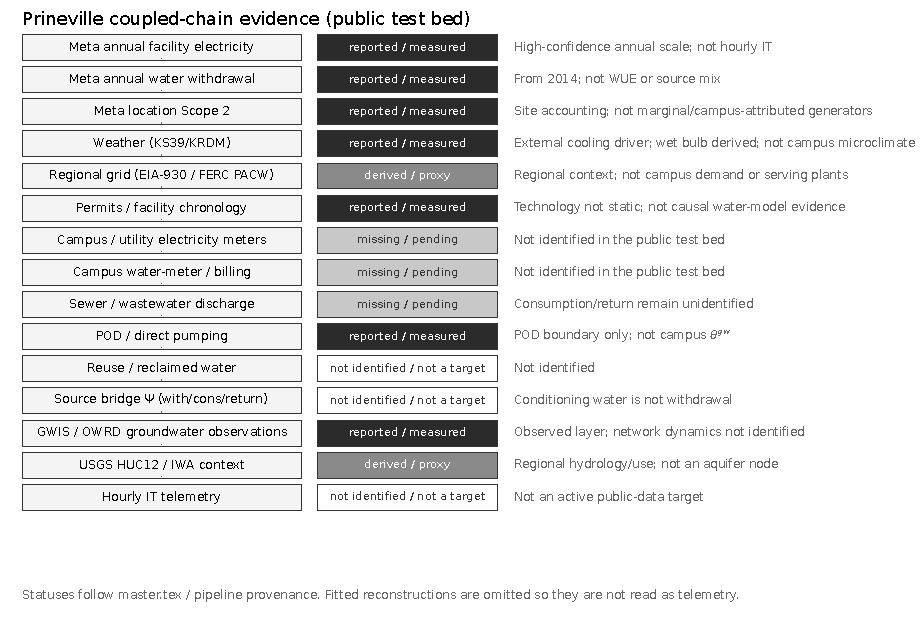
\includegraphics[width=0.98\linewidth]{img/fig_prineville_testbed_status.pdf}%
}{%
  \fbox{\begin{minipage}[c][2.55in][c]{0.92\linewidth}
  \centering
  \textbf{PLACEHOLDER --- Prineville empirical test-bed architecture and status}\\[0.7em]
  Suggested layers: Meta annual facility electricity / water / Scope 2
  $\rightarrow$ weather + regional grid + generation + permits
  $\rightarrow$ utility electricity + campus water/sewer
  $\rightarrow$ POD/pumping/reuse/discharge source accounting
  $\rightarrow$ GWIS/OWRD/USGS groundwater observations.\\[0.7em]
  Mark each stream as \Reported{}, \Measured{}, \Derived{}, \Proxy{},
  missing/pending, or not identified. Preserve the distinction between
  campus quantities, regional proxies, and groundwater observations.
  \end{minipage}}%
}
\caption{\textbf{Prineville as the integrated empirical test bed.}
Available public and requested data identify different portions of the
facility--water--grid--groundwater chain. Missing utility and source-accounting
quantities are shown explicitly rather than reconstructed as historical telemetry.}
\label{fig:prineville_testbed}
\end{figure}

% ================================================================
\section{Boundary rules: claims that must not be crossed}
% ================================================================

The following rules are canonical and should be treated as model constraints on interpretation:

\begin{enumerate}
\item \textbf{Regional quantities are not campus quantities:}
$E^{Meta}_{campus}\neq D^{PACW}\neq G^{Oregon}_{plants}$.
\item \textbf{Node/device power is not facility IT power.} Keep GPU/device $\rightarrow$ node/system $\rightarrow$ facility-IT boundaries explicit.
\item \textbf{PUE is derived.} Do not independently sample PUE and bottom-up cooling loads in a way that double counts facility overhead.
\item \textbf{WUE is not groundwater pumping.} Modeled conditioning-water use must pass through withdrawal/consumption/return and source-allocation accounting before entering a groundwater model.
\item \textbf{Withdrawal, consumption, return/discharge, reuse, and storage are distinct.} Do not combine them without a documented mass-balance relationship.
\item \textbf{Generator water is not direct site water.} Indirect electricity-water accounting remains a separate grid layer.
\item \textbf{Scarcity indices are not groundwater state.} HUC/AWARE/Aqueduct-style metrics are screening/impact indicators, not hydraulic head, storage, recharge, or firm local availability.
\item \textbf{Geographic overlap is not physical attribution.} Proximity does not identify a serving well, aquifer connection, generator, or water source.
\item \textbf{Same-data literature triangulation is not independent validation.} Independence must be stated explicitly for each benchmark.
\item \textbf{Simulation does not recover missing telemetry.} Scenario output can test counterfactuals but cannot become evidence of historical Meta operations.
\end{enumerate}

% ================================================================
\section{Validation philosophy and evidence ladder}
% ================================================================

Every model layer should pass the strongest validation available before it is allowed to influence planning decisions.

\begin{center}
\small
\begin{tabularx}{0.97\linewidth}{@{}p{0.18\linewidth}p{0.31\linewidth}Y@{}}
\toprule
\textbf{Validation level} & \textbf{Question} & \textbf{Project rule} \\
\midrule
Boundary / unit QC & Are quantities physically and dimensionally what we claim? & Mandatory before modeling. Missing is not zero; accounting identities are not predictive validation. \\
Reproduction & Can published code/data be reproduced in a pinned environment? & Preserve compatibility issues and numerical discrepancies; do not silently patch science. \\
Chronological holdout & Does the relationship transfer forward in time? & Prefer expanding/forward splits; do not random-split time-series claims. \\
Cross-regime / cross-workload & Does structure survive climate, workload, hardware, or operating regime changes? & Predeclare cells/holdouts where possible; do not select on outcomes. \\
Independent source/facility & Does a different dataset support the same structural dependency? & Strongest empirical support for generic structure; shared-data/shared-lineage evidence is triangulation only. \\
Decision replay & Does added fidelity change optimal decisions or prevent violations? & Final criterion for embedding complexity inside optimization. \\
\bottomrule
\end{tabularx}
\end{center}

The project freezes holdouts before translation/calibration whenever possible. The Meta 2023--2024 water holdout is a particularly important protected test set. Model complexity should not be added merely because a richer model fits benchmark telemetry better.

% ================================================================
\section{What is supported, what is provisional, and what is not identified}
% ================================================================

\begin{center}
\scriptsize
\begin{tabularx}{\linewidth}{@{}p{0.25\linewidth}p{0.20\linewidth}Y@{}}
\toprule
\textbf{Claim / quantity} & \textbf{Status} & \textbf{Current meaning} \\
\midrule
$P^{fac}=P^{IT}+P^{cool}+P^{aux}$ & \Strong & Supported by facility accounting and M100 measurement structure. \\
Weather-dependent facility overhead & \Strong & M100 chronological/within-month evidence; consistent with archetype physics. \\
IT-load dependence of accessory/cooling power & \Strong / Frontier QC pending & Frontier F1 beats constant baseline in all 9 folds; gap-safe energy audit still closing. \\
Planning intensity model $P^{fac}=P^{IT}PUE_k(\mathbf w)$ & \Partial & Highest-confidence current planning backbone candidate; annual Masanet/RNG gate still running. \\
$W^{cond}=E^{IT}WUE_k(\mathbf w)$ & \Partial & Identified facility-side conditioning-water intensity; annual validation pending. \\
IT$\times$weather interaction as mandatory term & Not required by M100 & $0/8$ folds achieve the predeclared $\ge5\%$ incremental threshold. \\
Measured M100 free-cooling flag as generic state & Not stably supported & Do not require it in planning model. \\
Generic operational dynamic state equation & \NotIdentified & Temporal memory exists, but tested recursive D1 is not validated. \\
Generic modern AI workload $\rightarrow P^{IT}$ & \NotIdentified & Experiment designed; no result yet. \\
Conditioning water $\rightarrow$ source withdrawal/return & \NotIdentified & Requires source shares, reuse/reclaimed supply, discharge/return and related accounting. \\
Groundwater share $\theta^{gw}$ & \NotIdentified & Direct POD reports are not the full campus source mix. \\
Pumping $\rightarrow$ groundwater causal response & \NotIdentified & First chronological empirical benchmark is next; recharge/background controls may be needed. \\
Dynamic groundwater network $(A,B_R,B_Q)$ & \NotIdentified & Target research model, not yet calibrated from Prineville. \\
Meta-specific marginal grid emissions/water & \NotIdentified & Regional averages/proxies are available; serving attribution and marginal dispatch are not. \\
Optimization / policy result & \NotIdentified & Requires validated response layers and decision-relevance testing. \\
\bottomrule
\end{tabularx}
\end{center}



% ----------------------------------------------------------------
% Living Figure 4: scientific gates and fidelity escalation.
% ----------------------------------------------------------------
\begin{figure}[!htbp]
\centering
\IfFileExists{img/fig_research_gates.pdf}{%
  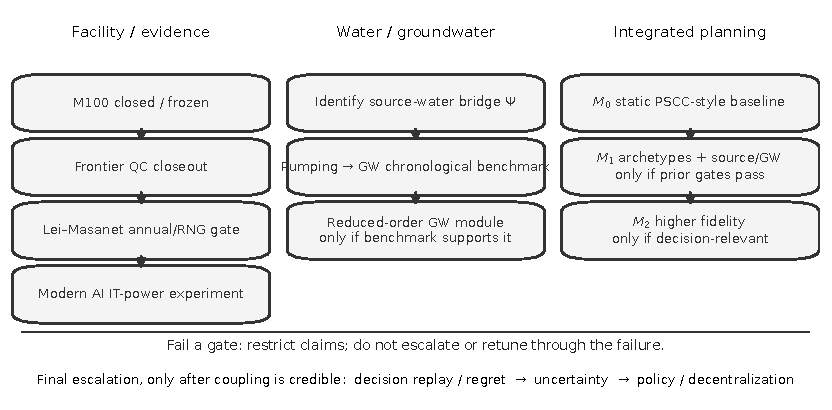
\includegraphics[width=0.97\linewidth]{img/fig_research_gates.pdf}%
}{%
  \fbox{\begin{minipage}[c][2.55in][c]{0.92\linewidth}
  \centering
  \textbf{PLACEHOLDER --- Scientific gating and model-fidelity path}\\[0.7em]
  Facility evidence: M100 closed $\rightarrow$ Frontier closeout
  $\rightarrow$ Lei--Masanet annual/RNG gate $\rightarrow$ modern AI IT-power gate.\\[0.5em]
  Water-resource evidence: source-water bridge $\rightarrow$
  pumping--groundwater benchmark $\rightarrow$ reduced groundwater network.\\[0.5em]
  Integration: $M_0$ static PSCC baseline $\rightarrow$
  $M_1$ validated archetypes + source water + groundwater $\rightarrow$
  $M_2$ higher fidelity only if decision-relevant.\\[0.5em]
  Final gate: decision replay/regret $\rightarrow$ uncertainty
  $\rightarrow$ policy/decentralization.
  \end{minipage}}%
}
\caption{\textbf{Research gates and escalation rule.}
Model fidelity increases only after the preceding empirical question is
resolved and only when added detail can affect planning decisions. Failed
gates restrict claims rather than triggering unconstrained model tuning.}
\label{fig:research_gates}
\end{figure}

% ================================================================
\section{Immediate scientific gates and stop rules}
% ================================================================

The project should advance through a small number of explicit gates rather than continue open-ended data/model expansion.

\begin{enumerate}
\item \textbf{Close the Lei--Masanet annual/RNG gate.} If it passes, freeze a clean climate--technology planning adapter with energy-weighted PUE/WUE and explicit water components. If it fails, retain the model only as qualitative archetype evidence.
\item \textbf{Close Frontier gap-safe QC.} Preserve the chronological IT-load result if pointwise metrics remain unchanged; do not claim thermal conservation beyond what the dataset supports.
\item \textbf{Run the modern AI IT-power experiment.} Determine whether a generic H100/B200 utilization map exists or whether hardware-class maps are required; quantify device$\rightarrow$system$\rightarrow$facility-IT boundary gaps.
\item \textbf{Run the Prineville pumping$\rightarrow$groundwater benchmark.} If antecedent pumping adds stable chronological skill, build a small reduced-order groundwater module. If not, add recharge/background groundwater controls before increasing complexity.
\item \textbf{Identify the site-water/source bridge.} Use available utility/POD/reuse/discharge evidence to map $W^{cond}$ and other site uses to withdrawal, consumption, return, and groundwater share. Do not use WUE as a substitute.
\item \textbf{Build the first archetype ensemble.} Use a small set of defensible climate/cooling technologies rather than one ``generic data center.'' Preserve joint energy--water parameter draws.
\item \textbf{Run the decision-relevance experiment.} Compare $M_0$ fixed coefficients, $M_1$ validated archetypes, and $M_2$ higher fidelity only if available. Measure regret, changed siting/source/cooling choices, groundwater/capacity violations, and equity outcomes.
\item \textbf{Only then add uncertainty and policy.} Introduce stochastic recharge/demand/energy scenarios, multi-sector endogenous allocation, and the J-WAFS policy/decentralization layer after the deterministic coupling is credible.
\end{enumerate}

\textbf{Stop rules.} M100 model development is closed. Do not turn the Masanet gate into a model-tuning exercise. Do not fit large black-box IT-power models before the nested simple experiment. Do not build a detailed groundwater simulator before the empirical pumping-response question is answered. Do not add facility dynamics to the planning model unless decision replay shows a material need.

% ================================================================
\section{Research contribution map}
% ================================================================

The project sits at the interface of mature literatures rather than replacing them.

\begin{center}
\scriptsize
\begin{tabularx}{\linewidth}{@{}p{0.20\linewidth}p{0.28\linewidth}Y@{}}
\toprule
\textbf{Literature / project layer} & \textbf{What is inherited} & \textbf{Project contribution / gap} \\
\midrule
LBNL / national accounting \cite{lbnl,siddik} & Aggregate energy/water envelopes, geography, system boundaries. & Use as envelope/context; not facility telemetry or dynamic groundwater. \\
M100 \cite{m100} & Measured internal facility structure and chronology. & Structural validation of weather/load/boundaries without coefficient transfer. \\
Lei--Masanet \cite{lei2022} & Joint climate/technology PUE/WUE physics and uncertainty. & Build a clean planning archetype adapter while preserving source-water uncertainty. \\
Frontier \cite{frontier} & Independent measured IT/accessory/thermal context. & Cross-facility support for load dependence; thermal/energy validation boundary. \\
Modern AI power datasets & Device/node/system power and utilization across H100/B200 and standardized workloads. & Identify the workload/hardware $\rightarrow$ IT-power block and boundary gaps. \\
Water-footprint / operational work \cite{li,gupta,waterwise} & Direct/indirect accounting, temporal signals, workload flexibility. & Endogenize environmental signals when decision-relevant rather than treating them all as exogenous coefficients. \\
PSCC \cite{pscc} & Static cost--carbon--water--equity siting backbone. & Replace static water treatment with source-resolved dynamic groundwater consequences. \\
Groundwater / hydro-economic models \cite{modflow,harou} & Pumping/recharge/state dynamics and multi-sector allocation. & Couple them to data-center workload/facility/source decisions in a tractable planning model. \\
J-WAFS \cite{jwa} & Groundwater security, infrastructure planning, policy mechanisms in water-stressed India. & Integrate validated facility/source demand with dynamic groundwater and decision/policy design. \\
\bottomrule
\end{tabularx}
\end{center}

% ================================================================
\section{Canonical project records and document governance}
% ================================================================

This document is the only manually maintained project-wide scientific narrative. Detailed implementation truth remains in machine-readable or experiment-specific artifacts.

\begin{center}
\scriptsize
\begin{tabularx}{0.97\linewidth}{@{}p{0.32\linewidth}Y@{}}
\toprule
\textbf{Record} & \textbf{Role} \\
\midrule
This document & Current scientific model, evidence, confidence, unresolved questions, and next gates. \\
\path{Meta_Prineville_Oregon_v3/} registries/reports & Site-specific source, quantity, model, QC, and validation accountability. \\
\path{other_sources/m100/results/}\newline\path{suitability_2021_v3_closure/} & Frozen M100 experimental evidence and machine-readable status. \\
\path{other_sources/masanet/} & Lei--Masanet/Frontier reproduction, audits, annual gate, adapter, and final status. \\
\path{other_sources/it_power/} & Modern AI power source audit and predeclared experiment. \\
J-WAFS proposal / PSCC paper & Immutable north-star proposal and static research baseline. \\
Archived handbook/glossary/meeting/early-model drafts & Historical reasoning and literature reference; not current specifications. \\
\bottomrule
\end{tabularx}
\end{center}

\textbf{Maintenance rule.} Update this document only after a result is supported by a canonical experiment report/status, an authoritative source, or an explicitly labeled preliminary result. Accepted changes should be merged into normal text. Use git history rather than permanent strike-through revisions. Keep TODOs short and tied to a specific scientific gate.

% ================================================================
\section{Current bottom line}
% ================================================================

The project now has a defensible scientific spine:
\[
\boxed{\begin{aligned}
\text{workload/hardware}
&\rightarrow P^{IT}\\
&\rightarrow \left\{
P^{fac}=P^{IT}PUE_k(\mathbf w,\theta_k),\;
W^{cond}=E^{IT}WUE_k(\mathbf w,\theta_k)
\right\}\\
&\rightarrow W^{with}\text{ by source}\\
&\rightarrow q^{gw}\\
&\rightarrow h_{m+1}=Ah_m+B_RR_m-B_Q(q^{ag}+q^{mun}+q^{dc})\\
&\rightarrow \text{siting, source choice, equity, and policy}.
\end{aligned}}
\]

The strongest completed empirical lesson is that the facility layer cannot be represented credibly by a weather-independent fixed efficiency. The strongest unresolved physical bridge is from modeled onsite conditioning water to actual source withdrawal and groundwater forcing. The strongest unresolved resource-system question is whether pumping produces stable predictive groundwater responses at the available spatial/temporal scale. The strongest eventual validation is whether richer facility/source/groundwater physics materially changes decisions relative to the static PSCC-style baseline.

That is the project question the remaining experiments should serve.

% ================================================================
\begin{thebibliography}{99}\small

\bibitem{jwa}
S. Amin and D. Deka,
``Protecting Community Groundwater Security: Network-Based Planning for Data Centers in Water-Stressed India,''
MIT J-WAFS proposal, 2026.

\bibitem{pscc}
R. Chen, D. Chauhan, N. Engelman Lado, and S. Amin,
``A Multi-Objective Linear Programming Framework for Sustainable and Equitable Data Center Siting,''
project manuscript / submitted to PSCC 2026.

\bibitem{m100}
A. Borghesi et al.,
``M100 ExaData: a Data Collection Campaign on the CINECA's Marconi100 Tier-0 Supercomputer,''
\emph{Scientific Data}, vol. 10, art. 288, 2023.
\href{https://doi.org/10.1038/s41597-023-02174-3}{doi:10.1038/s41597-023-02174-3}.

\bibitem{frontier}
J. Sun, Z. Gao, D. Grant, et al.,
``Energy Dataset of Frontier Supercomputer for Waste Heat Recovery,''
\emph{Scientific Data}, vol. 11, art. 1077, 2024.
\href{https://doi.org/10.1038/s41597-024-03913-w}{doi:10.1038/s41597-024-03913-w}.

\bibitem{lei2022}
N. Lei and E. Masanet,
``Climate- and Technology-Specific PUE and WUE Estimations for U.S. Data Centers Using a Hybrid Statistical and Thermodynamics-Based Approach,''
\emph{Resources, Conservation and Recycling}, vol. 182, 106323, 2022.
\href{https://doi.org/10.1016/j.resconrec.2022.106323}{doi:10.1016/j.resconrec.2022.106323}.

\bibitem{lbnl}
A. Shehabi et al.,
``2024 United States Data Center Energy Usage Report,''
Lawrence Berkeley National Laboratory, 2024.
\href{https://doi.org/10.71468/P1WC7Q}{doi:10.71468/P1WC7Q}.

\bibitem{siddik}
M. A. B. Siddik, A. Shehabi, and L. T. Marston,
``The Environmental Footprint of Data Centers in the United States,''
\emph{Environmental Research Letters}, vol. 16, 064017, 2021.
\href{https://doi.org/10.1088/1748-9326/abfba1}{doi:10.1088/1748-9326/abfba1}.

\bibitem{li}
P. Li, J. Yang, M. A. Islam, and S. Ren,
``Making AI Less `Thirsty': Uncovering and Addressing the Secret Water Footprint of AI Models,''
arXiv:2304.03271, 2023/2024.

\bibitem{gupta}
P. Sen Gupta, M. R. Hossen, P. Li, S. Ren, and M. A. Islam,
``A Dataset for Research on Water Sustainability,''
arXiv:2405.17469, 2024.

\bibitem{waterwise}
Y. Jiang, R. Basu Roy, R. Kanakagiri, and D. Tiwari,
``WaterWise: Co-optimizing Carbon- and Water-Footprint Toward Environmentally Sustainable Cloud Computing,''
\emph{PPoPP}, 2025.
\href{https://doi.org/10.1145/3710848.3710891}{doi:10.1145/3710848.3710891}.

\bibitem{modflow}
C. D. Langevin et al.,
``MODFLOW 6 Modular Hydrologic Model,''
U.S. Geological Survey software release.

\bibitem{harou}
J. J. Harou et al.,
``Hydro-Economic Models: Concepts, Design, Applications, and Future Prospects,''
\emph{Journal of Hydrology}, vol. 375, pp. 627--643, 2009.
\href{https://doi.org/10.1016/j.jhydrol.2009.06.037}{doi:10.1016/j.jhydrol.2009.06.037}.

\bibitem{isoPUE}
ISO/IEC 30134-2:2026,
``Information technology---Data centres key performance indicators---Part 2: Power usage effectiveness (PUE).''

\bibitem{isoWUE}
ISO/IEC 30134-9:2022,
``Information technology---Data centres key performance indicators---Part 9: Water usage effectiveness (WUE).''

\end{thebibliography}

\end{document}
